\chapter{The Internal Structure of the Emergent Language (RQ1)}
\label{ch:experimental}

This chapter tests the first research question: whether and how the concentration parameter $\alpha$ of the Zipfian input distribution shapes the internal structure of the emergent language. We look at three complementary aspects of that structure. Section~\ref{sec:rq1-setup} describes the experimental setup. Section~\ref{sec:rq1-adoption-count} measures how many abstractions end up adopted into the vocabulary at each $\alpha$, which tells us how large the emergent vocabulary is. Section~\ref{sec:rq1-compression-dynamics} looks at how the emergent language compresses over training, through the evolution of message length and reconstruction accuracy. Section~\ref{sec:rq1-mdl-vs-frequency} asks what governs which candidate gets adopted when frequency and MDL diverge, and what this tells us about the specific pressure PACE encodes. Section~\ref{sec:rq1-discussion} closes with the interpretive picture that emerges across the three analyses.

\section{Experimental Setup}
\label{sec:rq1-setup}

The experimental campaign for RQ1 covers a grid of 20 seeds by 21 $\alpha$ values equally spaced between 0.00 and 3.00 in steps of 0.15, for a total of 420 training runs. Every run uses the same PACE configuration described in Chapter~\ref{ch:pace}, with the same architectural and hyperparameter choices reported in Appendix~\ref{ch:apdb}. Only the concentration parameter $\alpha$ and the seed vary across runs, and the seed controls both the random initialisation of the neural agents and the permutation used to build the Zipfian dataset. This means that any effect we observe in the emergent language can be attributed to $\alpha$ (through the aggregate statistics across seeds) or to seed-specific variation (through the spread within an $\alpha$), and not to differences in the training procedure.

For each run we record the abstraction tracker and the step-level log produced during training. The step-level log identifies, for every proposal step, which candidates were shortlisted by the MDL scoring rule and which candidate was adopted. This is the raw material that feeds the analyses that follow.

We characterise the internal structure of the emergent language at each $\alpha$ along three complementary metrics. The first is the adoption count: the total number of abstractions that end up in the abstraction tracker at the end of training. Because the maximum number of proposal steps is fixed, and each step can adopt at most one candidate, the adoption count has a fixed upper bound. Its value at each $\alpha$ tells us how fully the vocabulary develops under that input distribution.

The second is the compression dynamics of the emergent language during training. At each proposal step, we record the mean length of the messages the speaker produces on the training set. Because adopting an abstraction replaces a multi-token subsequence with a single abstraction, mean message length is a direct measure of how much the emergent language has compressed. Tracking mean message length across proposal steps produces a curve for each $\alpha$, and comparing these curves across $\alpha$ values tells us whether more concentrated distributions lead to faster or slower compression.

The third is the signal that drives adoption. At every proposal step the system produces a shortlist of candidate sub-sequences and deterministically adopts the candidate with the highest MDL score. Comparing this candidate with the one ranked highest by raw frequency tells us how often the compression-oriented MDL rule differs from a frequency-only rule, and whether that relationship changes with $\alpha$.

\section{How Many Abstractions Are Adopted}
\label{sec:rq1-adoption-count}

The most direct measure of the internal structure of the emergent language is the size of the adopted vocabulary at the end of training. For each combination of $\alpha$ and seed, we count the number of distinct abstractions that end up adopted into the library over the course of training, and we aggregate across seeds to get a mean and a spread at each $\alpha$.

\begin{figure}[htbp]
    \centering
    \IfFileExists{images/adoption_vs_alpha.png}{%
        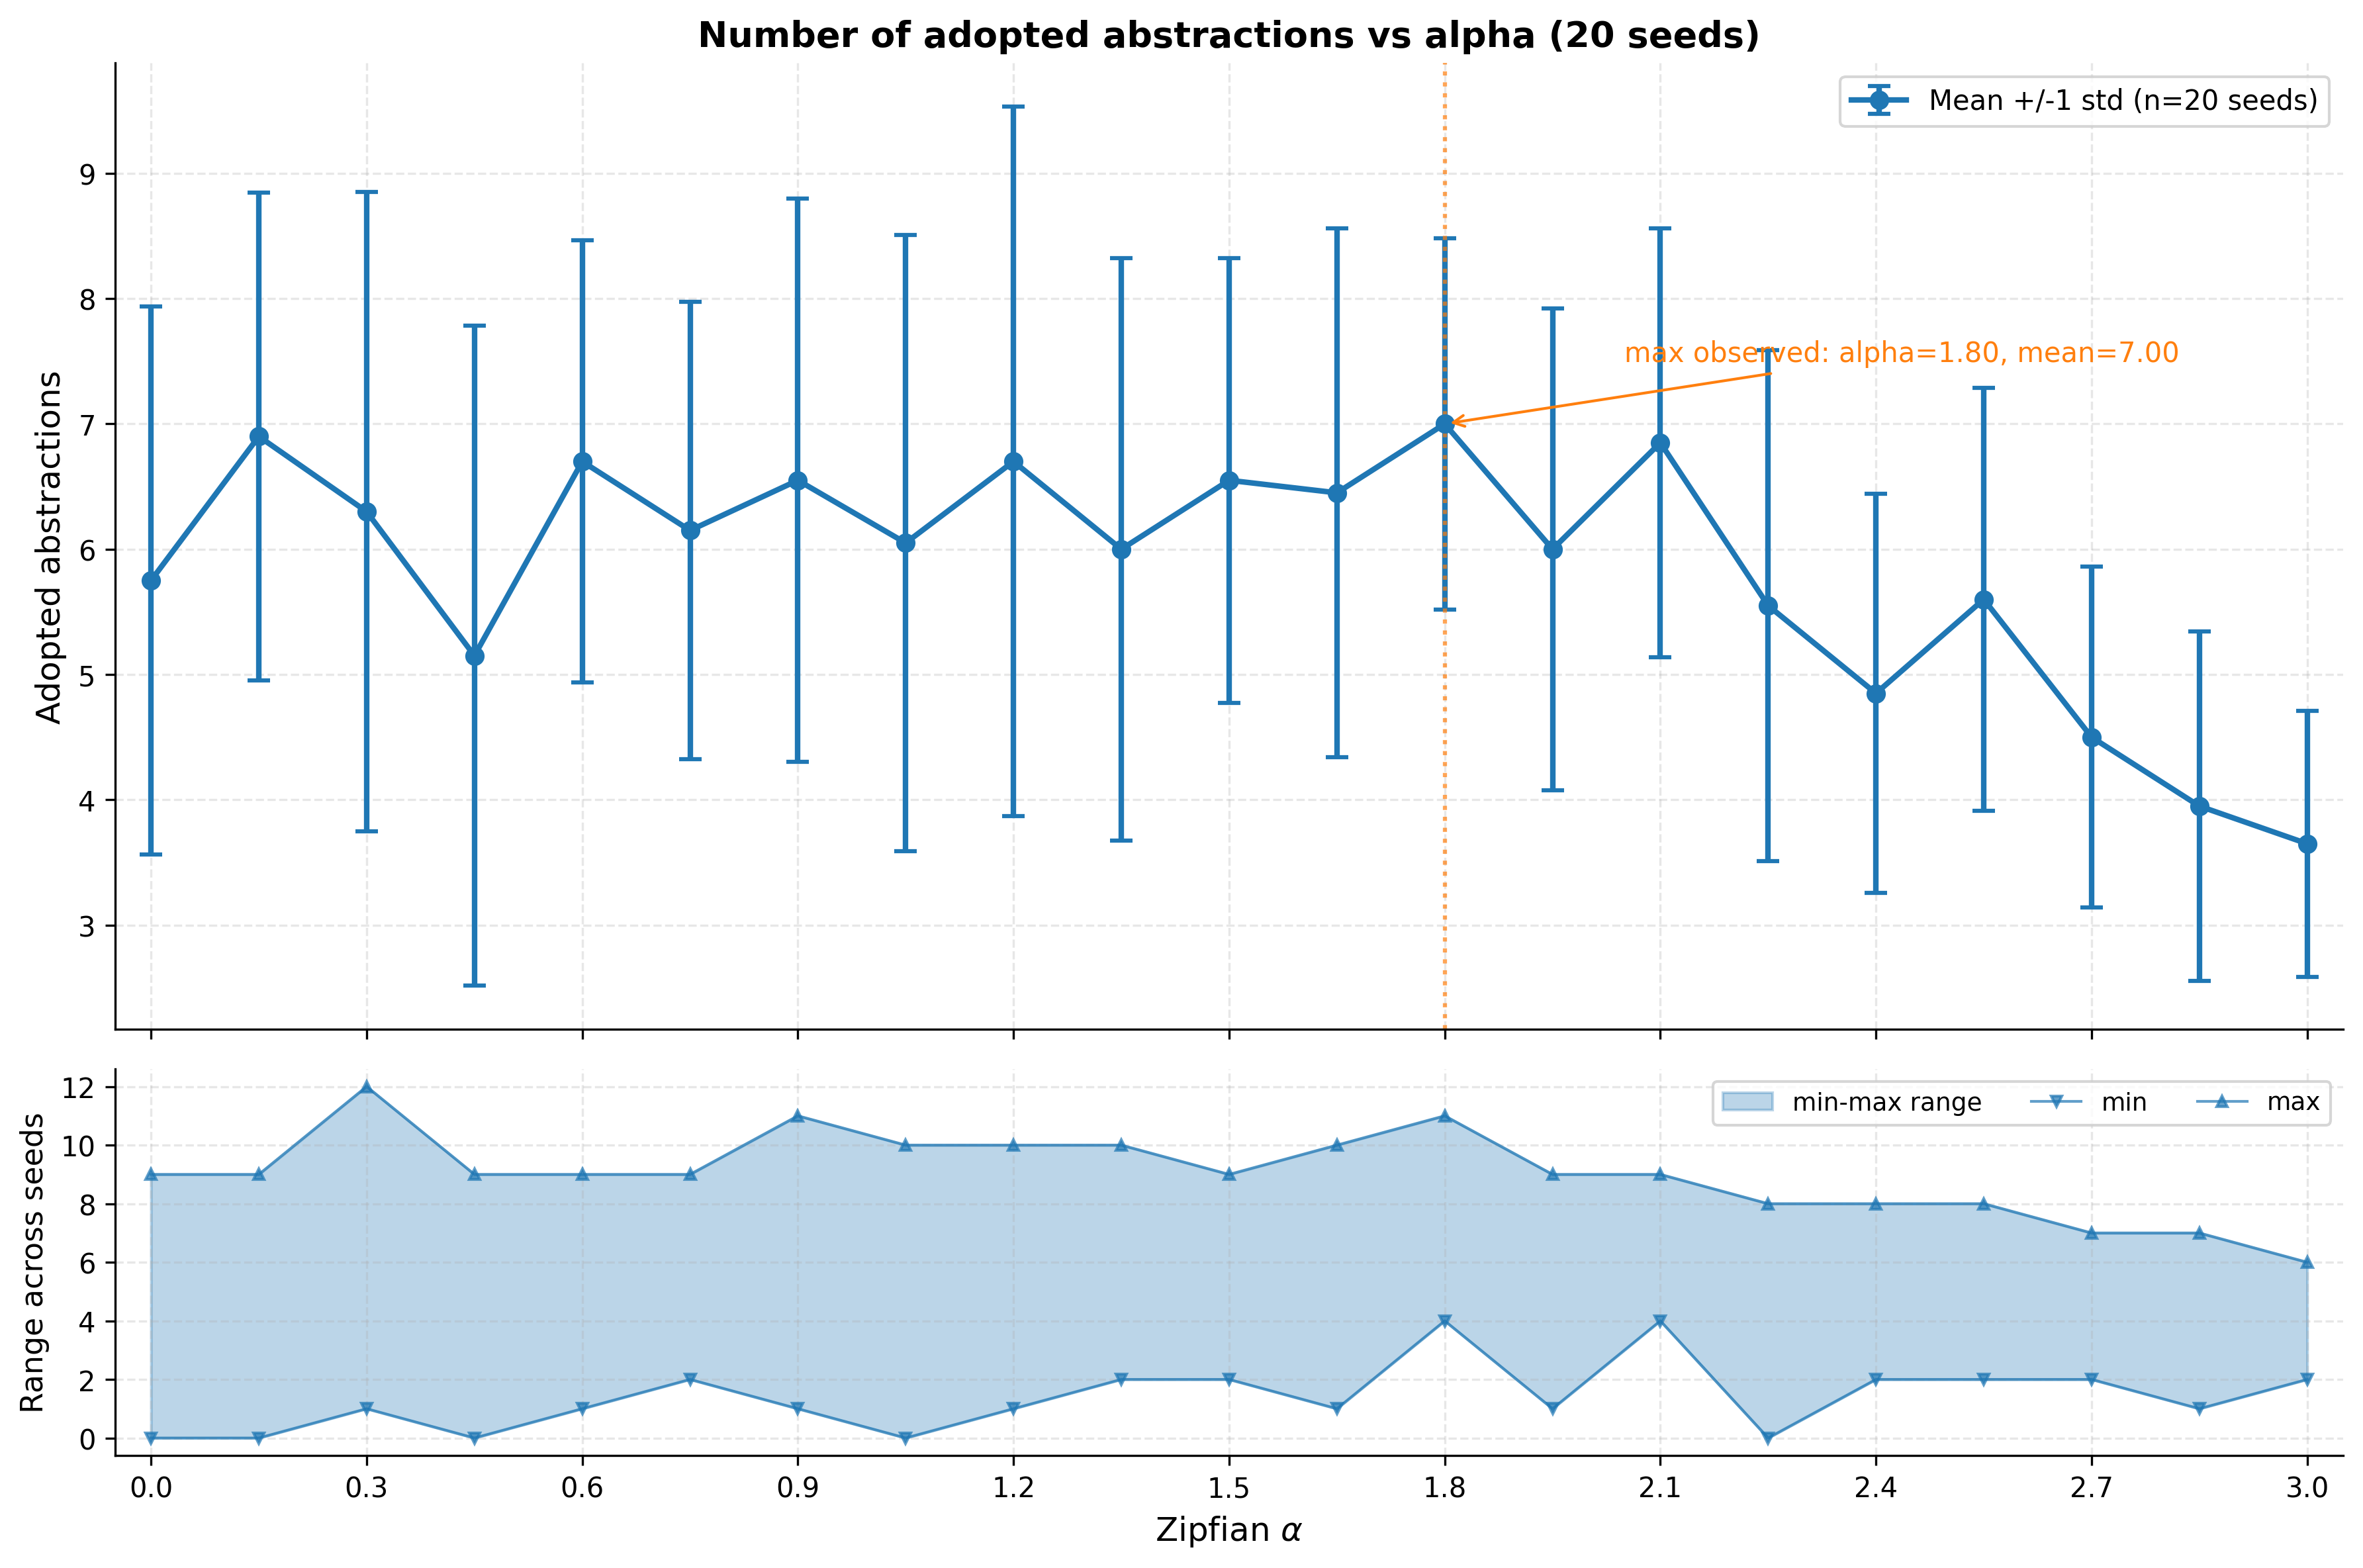
\includegraphics[width=0.95\textwidth]{images/adoption_vs_alpha.png}%
    }{%
        \fcolorbox{red}{white}{\parbox[c][0.14\textheight][c]{0.9\textwidth}{\centering\textcolor{red}{Placeholder figure\\\texttt{\detokenize{images/adoption_vs_alpha.png}}}}}%
    }
    \caption{Number of adopted abstractions as a function of $\alpha$. The upper panel shows the mean and standard deviation across 20 seeds, and the lower panel shows the min--max range. ``Adopted'' means abstractions added to the library by the deterministic MDL rule, distinct from the larger set of candidates considered at each step.}
    \label{fig:rq1-adoption-vs-alpha}
\end{figure}

The curve of Figure~\ref{fig:rq1-adoption-vs-alpha} shows a pattern that separates three regimes across the $\alpha$ range.

In the low-$\alpha$ regime ($\alpha$ from 0.00 to about 0.45), the mean number of adopted abstractions fluctuates around 5 to 7, with a large standard deviation across seeds. The dispersion is not surprising: at these $\alpha$ values the training distribution is close to uniform and no pair of shapes stands out as clearly more frequent than another. Different seeds therefore produce different candidate pools and converge on different libraries, all of comparable size; the specific composition of each library reflects which pairs happen to have been sampled more often by chance rather than any systematic property of the input distribution.

In the intermediate-$\alpha$ regime ($\alpha$ from about 0.60 to 2.10), the mean number of adopted abstractions stabilises in the same 5 to 7 range but with a clear structural signal beneath the noise. The maximum of the curve is at $\alpha = 1.80$, where the mean rises to 7.00. This is the point where the training distribution provides the best combination of two conditions: on one hand, a small number of pairs at the top of the ranking are sampled often enough to yield strong statistical evidence for their abstractability; on the other hand, enough scenes down the rank remain represented to provide the diversity that keeps other candidates competitive. Below this value the input is too uniform to favour any specific pattern strongly; above it, the distribution becomes so concentrated that most of the ranking is starved of samples.

In the high-$\alpha$ regime (from $\alpha = 2.25$ upwards), the mean number of adopted abstractions falls rapidly, reaching about 3.6 at $\alpha = 3.00$. Alongside the mean drop, the min--max range in the lower panel of Figure~\ref{fig:rq1-adoption-vs-alpha} also contracts: the maximum observed across seeds falls from around 10 to 11 abstractions in the intermediate regime down to 6 to 8 abstractions at the top of the $\alpha$ range. In this regime the training distribution is so concentrated that only a handful of pairs at the top of the ranking see any meaningful frequency. The pool runs out of high-frequency sub-sequences that are worth adopting, and the resulting library is consequently smaller.

The three-regime pattern is important for what follows. The intermediate regime, from about $\alpha = 0.60$ to $\alpha = 2.10$, is where the emergent language is at its most developed, with the largest and most stable vocabularies. The low-$\alpha$ regime is where library composition is mostly noise-driven, and the high-$\alpha$ regime is where the input distribution starts to starve the vocabulary. RQ2 and RQ3 will show, in Chapters~\ref{ch:rq2} and~\ref{ch:rq3}, that these regimes leave distinct signatures on how populations relate to each other and on how they communicate under mismatch.

The aggregate counts become more interpretable when we look at the abstractions themselves. Figure~\ref{fig:rq1-abstraction-gallery-alpha-180} shows the full set of 19 candidate abstractions proposed during training for one representative population (seed 42 at $\alpha = 1.80$), each rendered as a 9-by-9 grid showing the shape it would draw on an empty grid. Green frames mark adopted abstractions; grey frames mark other candidates. Both groups contain recognisable structural motifs (vertical bars, small blocks, corner shapes) rather than arbitrary primitive strings, so the MDL ranking is not filtering out noise but choosing between competing meaningful patterns. The adopted abstractions are the candidates that offer the greatest compression under the MDL rule: adoption depends on repeated usefulness, not only on visual recognisability.

\begin{figure}[htbp]
    \centering
    \IfFileExists{images/abstraction_gallery_alpha_1.80.png}{%
        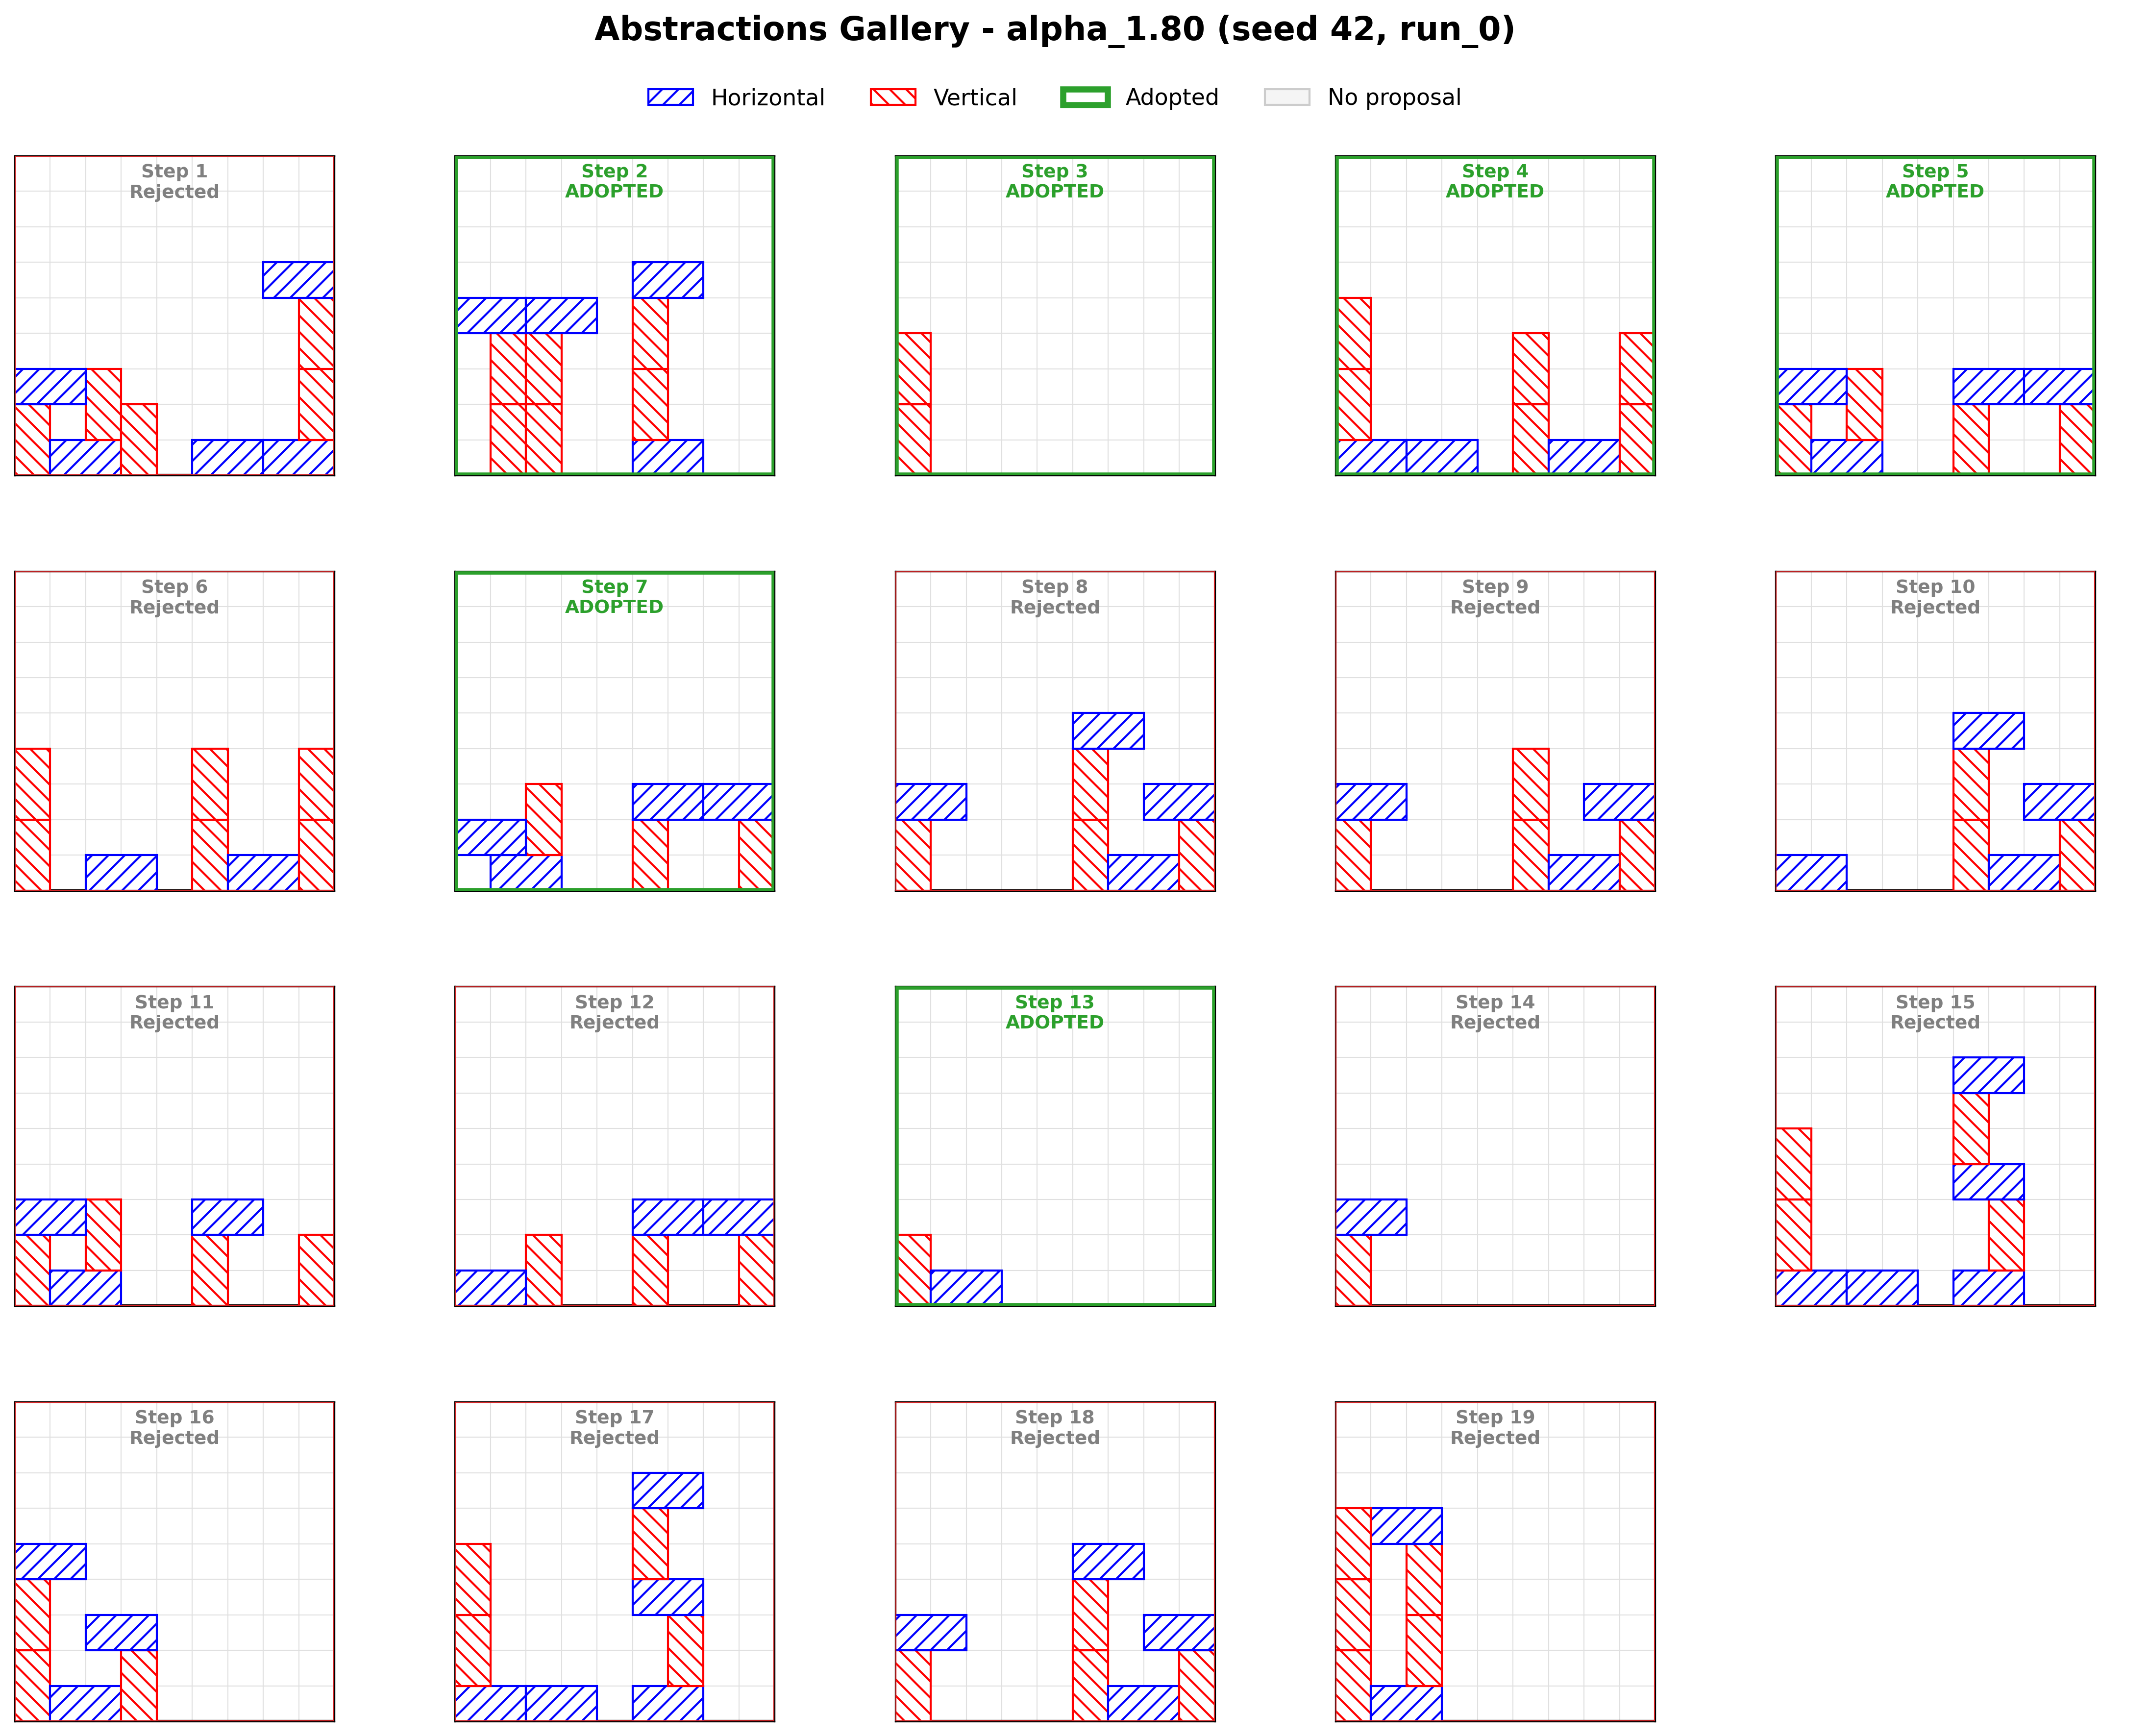
\includegraphics[width=0.95\textwidth]{images/abstraction_gallery_alpha_1.80.png}%
    }{%
        \fcolorbox{red}{white}{\parbox[c][0.14\textheight][c]{0.9\textwidth}{\centering\textcolor{red}{Placeholder figure\\\texttt{\detokenize{images/abstraction_gallery_alpha_1.80.png}}}}}%
    }
    \caption{Gallery of the abstractions adopted by seed 42 at $\alpha = 1.80$, shown as 9-by-9 grid visualisations. Each cell shows one adopted abstraction as it would be executed on an empty grid, giving a concrete picture of the patterns selected by the MDL rule for compression.}
    \label{fig:rq1-abstraction-gallery-alpha-180}
\end{figure}

\section{How the Emergent Language Compresses Over Training}
\label{sec:rq1-compression-dynamics}

A second aspect of the internal structure of the emergent language is how it evolves during training. Two quantities are informative here: the mean length of the messages the speaker produces, which measures how compressed the emergent language is at each step, and the reconstruction accuracy on the held-out test set, which measures how well the two agents understand each other. Every time a new abstraction is adopted, the corresponding subsequence of primitives in the messages gets replaced by a single abstraction, and the mean length drops.

\begin{figure}[htbp]
    \centering
    \IfFileExists{images/dynamics_combined_length.png}{%
        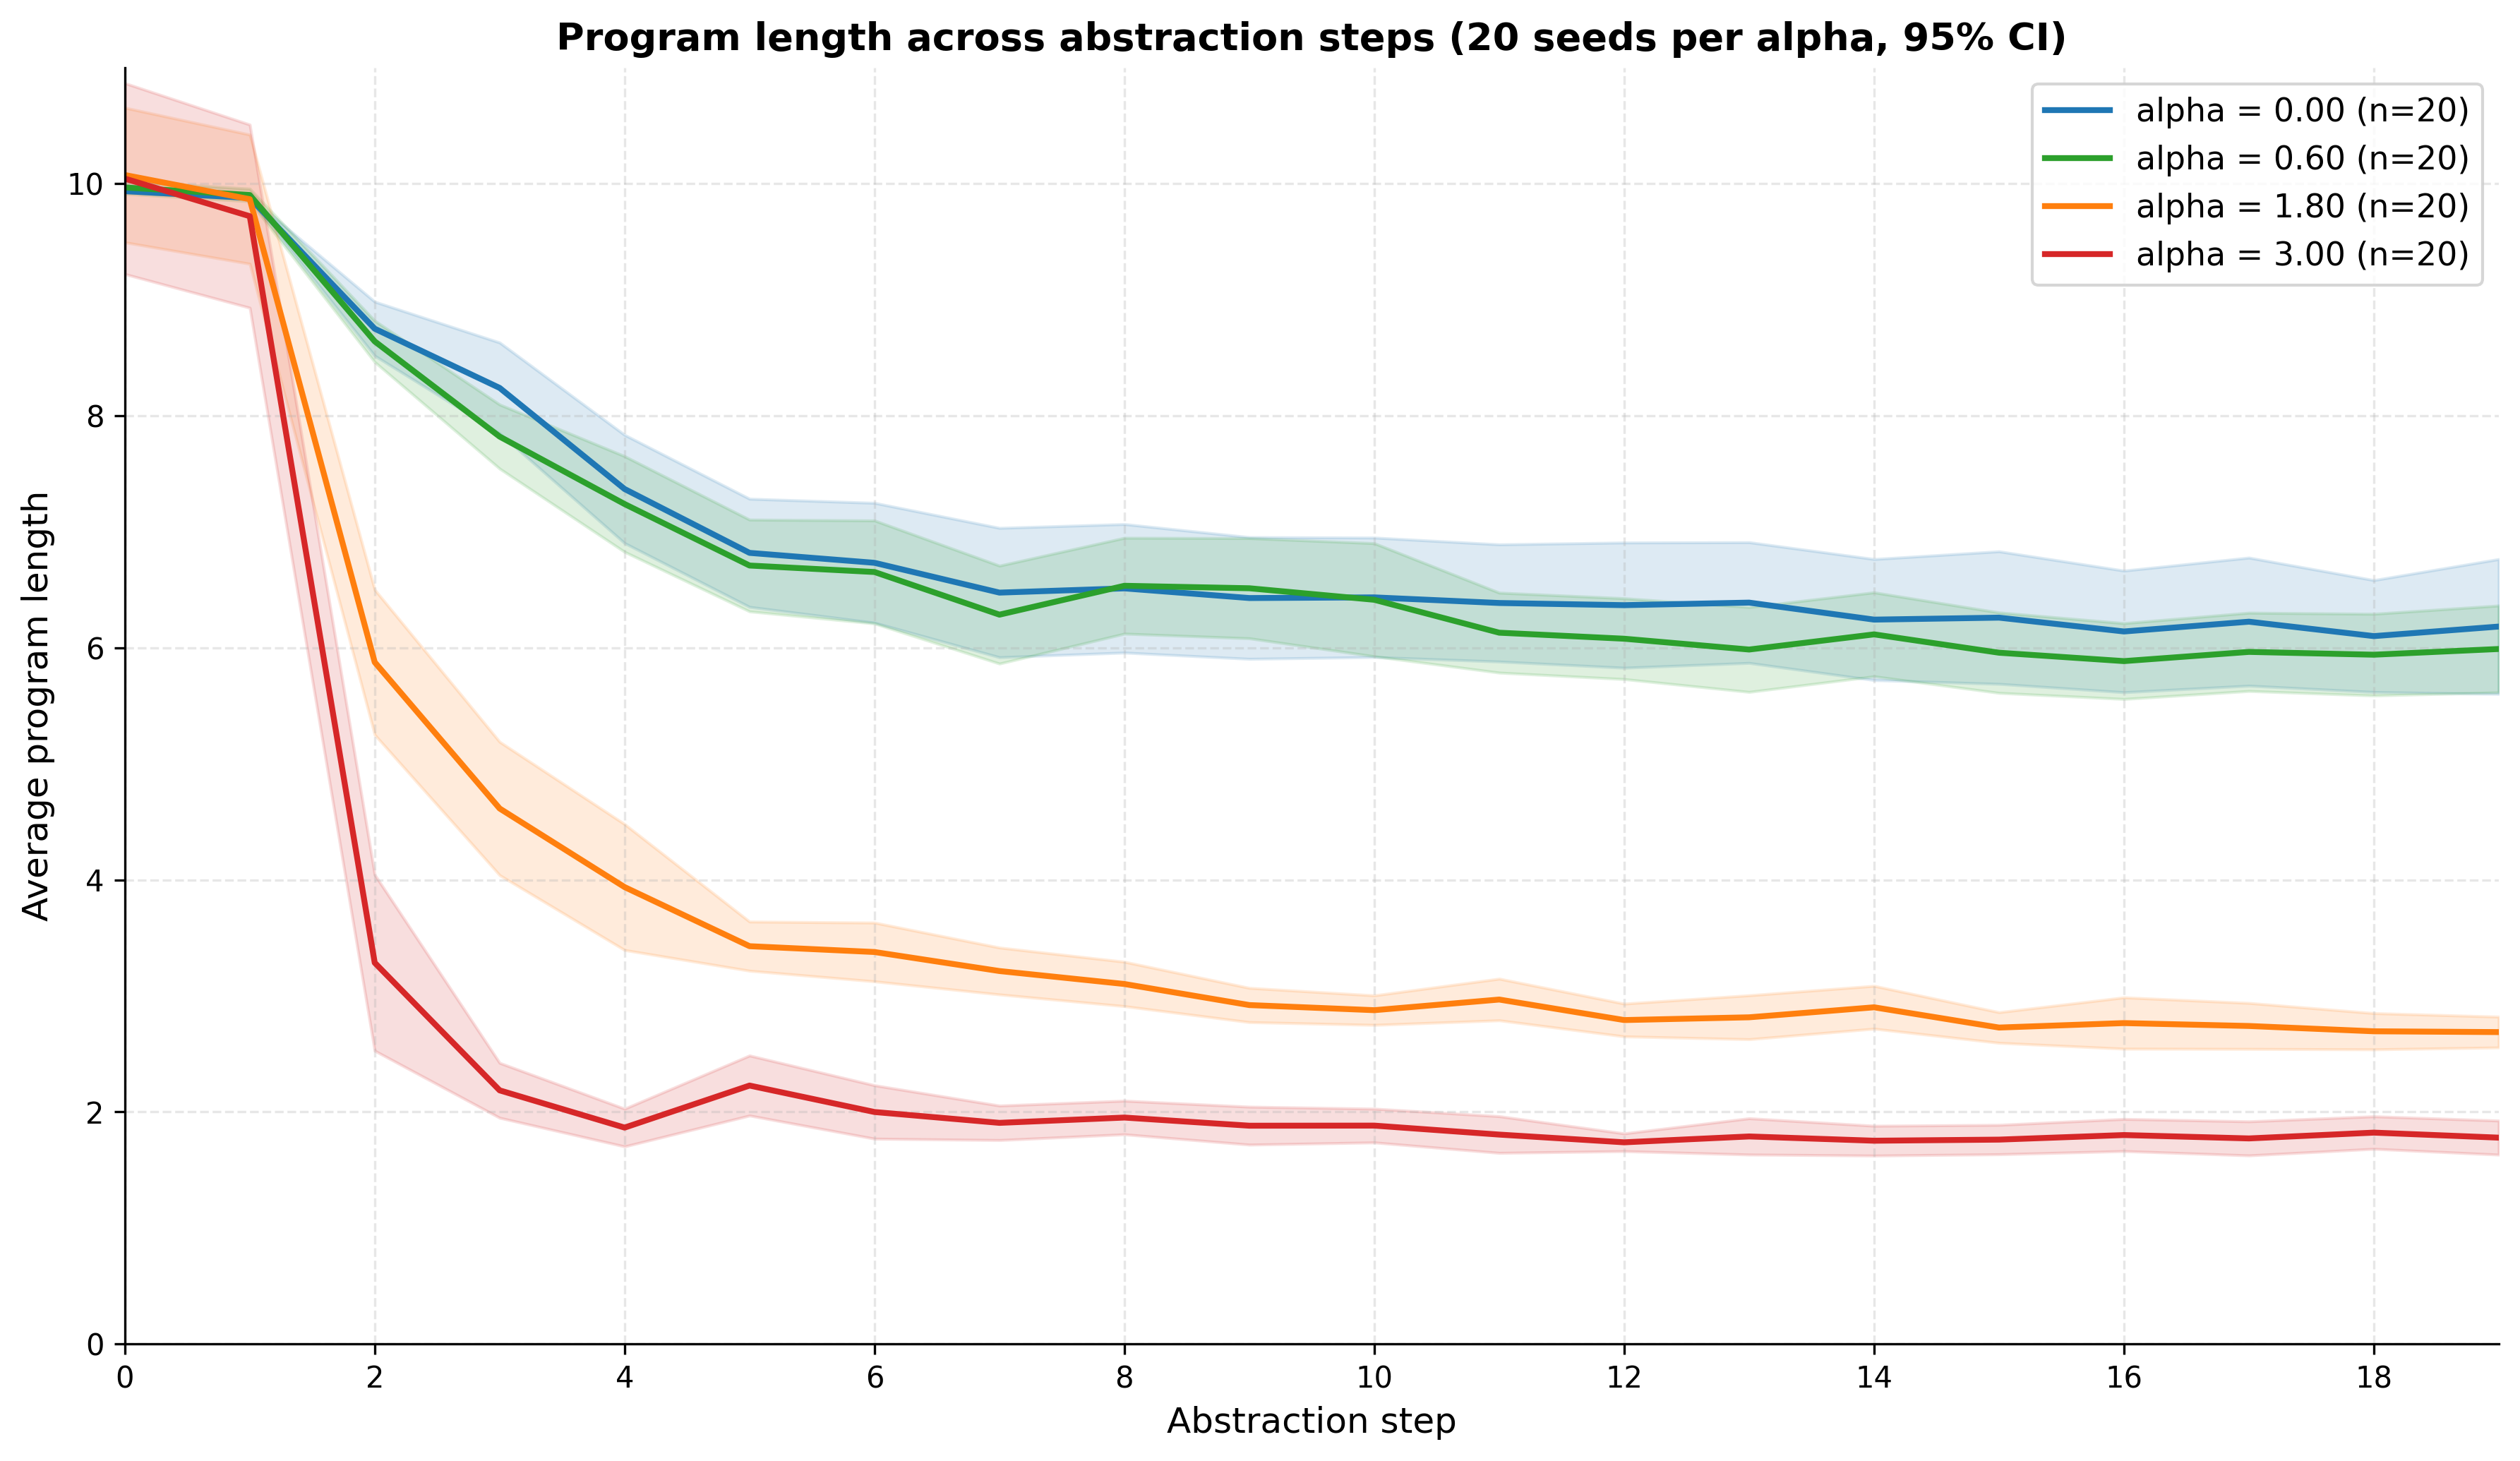
\includegraphics[width=0.95\textwidth]{images/dynamics_combined_length.png}%
    }{%
        \fcolorbox{red}{white}{\parbox[c][0.14\textheight][c]{0.9\textwidth}{\centering\textcolor{red}{Placeholder figure\\\texttt{\detokenize{images/dynamics_combined_length.png}}}}}%
    }
    \caption{Mean message length across proposal steps for representative $\alpha$ values ($0.00$, $0.60$, $1.80$, and $3.00$), showing the compression dynamics over training.}
    \label{fig:rq1-dynamics-length}
\end{figure}

\begin{figure}[htbp]
    \centering
    \IfFileExists{images/dynamics_combined_accuracy.png}{%
        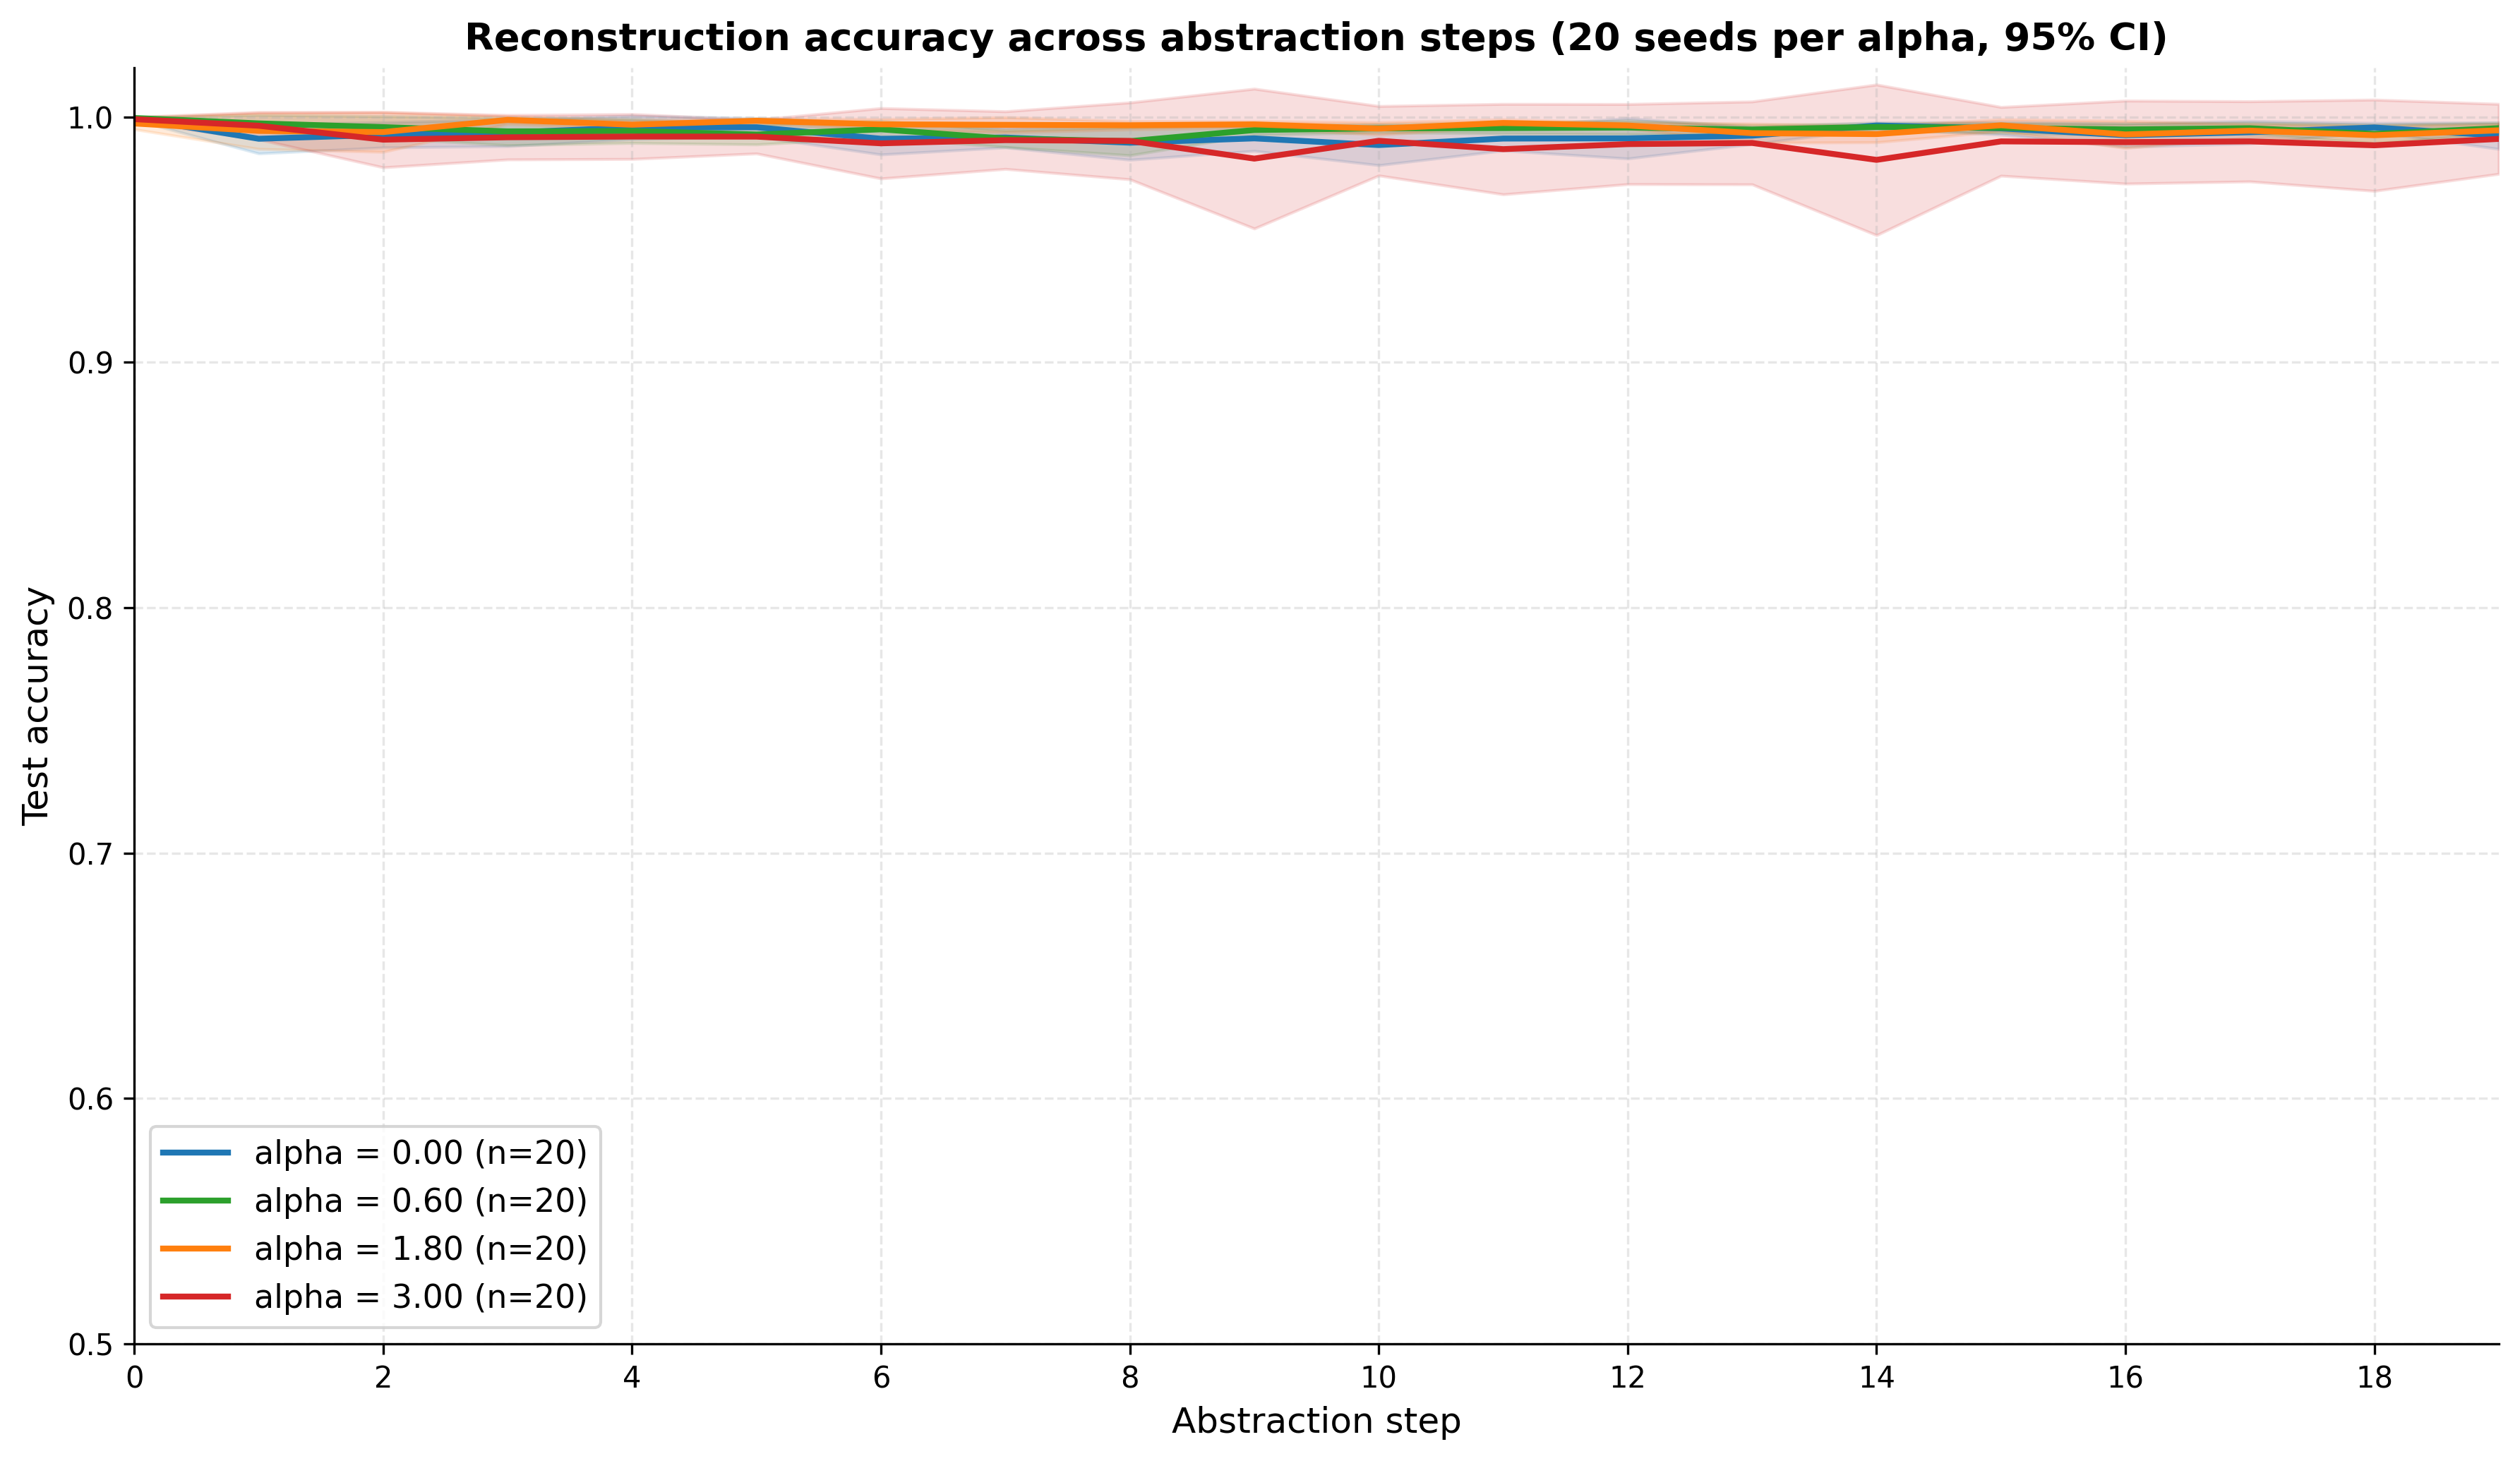
\includegraphics[width=0.95\textwidth]{images/dynamics_combined_accuracy.png}%
    }{%
        \fcolorbox{red}{white}{\parbox[c][0.14\textheight][c]{0.9\textwidth}{\centering\textcolor{red}{Placeholder figure\\\texttt{\detokenize{images/dynamics_combined_accuracy.png}}}}}%
    }
    \caption{Reconstruction accuracy on the test set across proposal steps for the same representative $\alpha$ values as Figure~\ref{fig:rq1-dynamics-length}.}
    \label{fig:rq1-dynamics-accuracy}
\end{figure}

Figure~\ref{fig:rq1-dynamics-length} shows the message-length curves for four representative $\alpha$ values. All curves start at nearly the same length, because step 0 precedes abstraction adoption and every scene is still written in primitives. The trajectories separate once abstractions begin to be adopted: $\alpha = 0.00$, $\alpha = 0.60$, and $\alpha = 1.80$ compress substantially, whereas $\alpha = 3.00$ remains higher throughout. This follows directly from Section~\ref{sec:rq1-adoption-count}. At $\alpha = 3.00$ fewer abstractions are adopted, leaving fewer opportunities to replace primitive subsequences with single tokens.

The three $\alpha$ values in the intermediate regime, meanwhile, produce similar amounts of compression by the end of training. The mean length settles at comparable values regardless of whether the training distribution was uniform ($\alpha = 0.00$) or moderately concentrated ($\alpha = 0.60$ and $\alpha = 1.80$). The compression that PACE achieves at these $\alpha$ values does not depend strongly on the concentration, only on the fact that there are enough proposal steps and enough scenes to provide useful candidate sub-sequences.

Figure~\ref{fig:rq1-dynamics-accuracy} shows the accuracy curves for the same four $\alpha$ values. The accuracy is close to 1.00 at step 0 and remains high throughout training in all four cases. The reason is that PACE trains the neural agents for many gradient updates between proposal phases, and the abstractions that are proposed at each phase are ones that MDL identifies as compressing the current messages well; they are not disruptive replacements but transparent shortcuts. Accuracy is therefore not the aspect that separates the $\alpha$ values from each other; what separates them is how quickly and how far the emergent language can compress before running out of exploitable patterns. The two curves together confirm that the concentration regimes do not differ in whether the agents can communicate, but in how efficiently they do so. All four settings reach reliable communication; only the intermediate ones do so with a compact vocabulary. This raises a further question: how often does the deterministic MDL rule select a different candidate from raw frequency alone? The next section addresses that.

\section{What Governs Adoption: MDL Score vs Raw Frequency}
\label{sec:rq1-mdl-vs-frequency}

The last analysis of this chapter looks at a specific mechanistic question. At each proposal step, the system produces a shortlist of candidate sub-sequences and selects one of them as a new abstraction. The rule PACE uses for this selection is deterministic: the candidate that maximises the MDL score wins. The MDL score combines the frequency of the sub-sequence with its length minus one. Because a long and frequent sub-sequence scores highly under both MDL and raw frequency, the two rankings can agree, but they are not equivalent.

But there is a natural question: how often does this MDL-optimal candidate coincide with the candidate that has the highest raw frequency? If the two coincide most of the time, then in practice PACE's adoption decisions look indistinguishable from a frequency-based rule. To test this, we compare the MDL top-ranked candidate with the raw-frequency top-ranked candidate at every adoption step across the 420 runs.

In 566 of the 724 adoption steps (78.2\%, or roughly four out of five), the MDL top-ranked candidate was different from the raw-frequency top-ranked candidate. In about four out of five adoption decisions, therefore, the chosen candidate diverges from what raw frequency alone would predict. The correlation between the adoption pattern and raw frequency is not statistically significant on the aggregate: the Spearman correlation is close to zero. What gets chosen instead is the candidate that scores highest under the MDL rule, showing that the compression pressure is empirically distinct from a frequency-only rule.

The distributional version of this comparison is reported in Appendix~\ref{ch:apdd}: at $\alpha = 1.80$, the MDL landscape shifts away from the uniform baseline, with fewer unique subsequences but systematically stronger top-ranked candidates. In the main text, the clearest way to see the mechanism is not another aggregate distribution, but a single proposal step where the two rankings disagree.

To make this even more concrete, Figures~\ref{fig:rq1-frequency-snapshot-alpha-180-step-06} and~\ref{fig:rq1-mdl-snapshot-alpha-180-step-06} show a snapshot at a single proposal step during training on the $\alpha = 1.80$ dataset. Both figures show the same set of candidate subsequences at that step, but ordered by two different criteria. Figure~\ref{fig:rq1-frequency-snapshot-alpha-180-step-06} orders them by raw frequency in the training data; Figure~\ref{fig:rq1-mdl-snapshot-alpha-180-step-06} orders them by MDL score. In both figures, the candidate adopted at that step is highlighted in green. In the MDL-ordered plot, the adopted candidate is at the top of the ranking (or tied with the top). In the frequency-ordered plot, this is not the case: the adopted candidate can sit several positions below the frequency top-ranked one. The snapshot is a visual example of the disagreement measured by the 78.2\% statistic reported above.

\begin{figure}[htbp]
    \centering
    \IfFileExists{images/frequency_snapshot_alpha_1.80_step_06.png}{%
        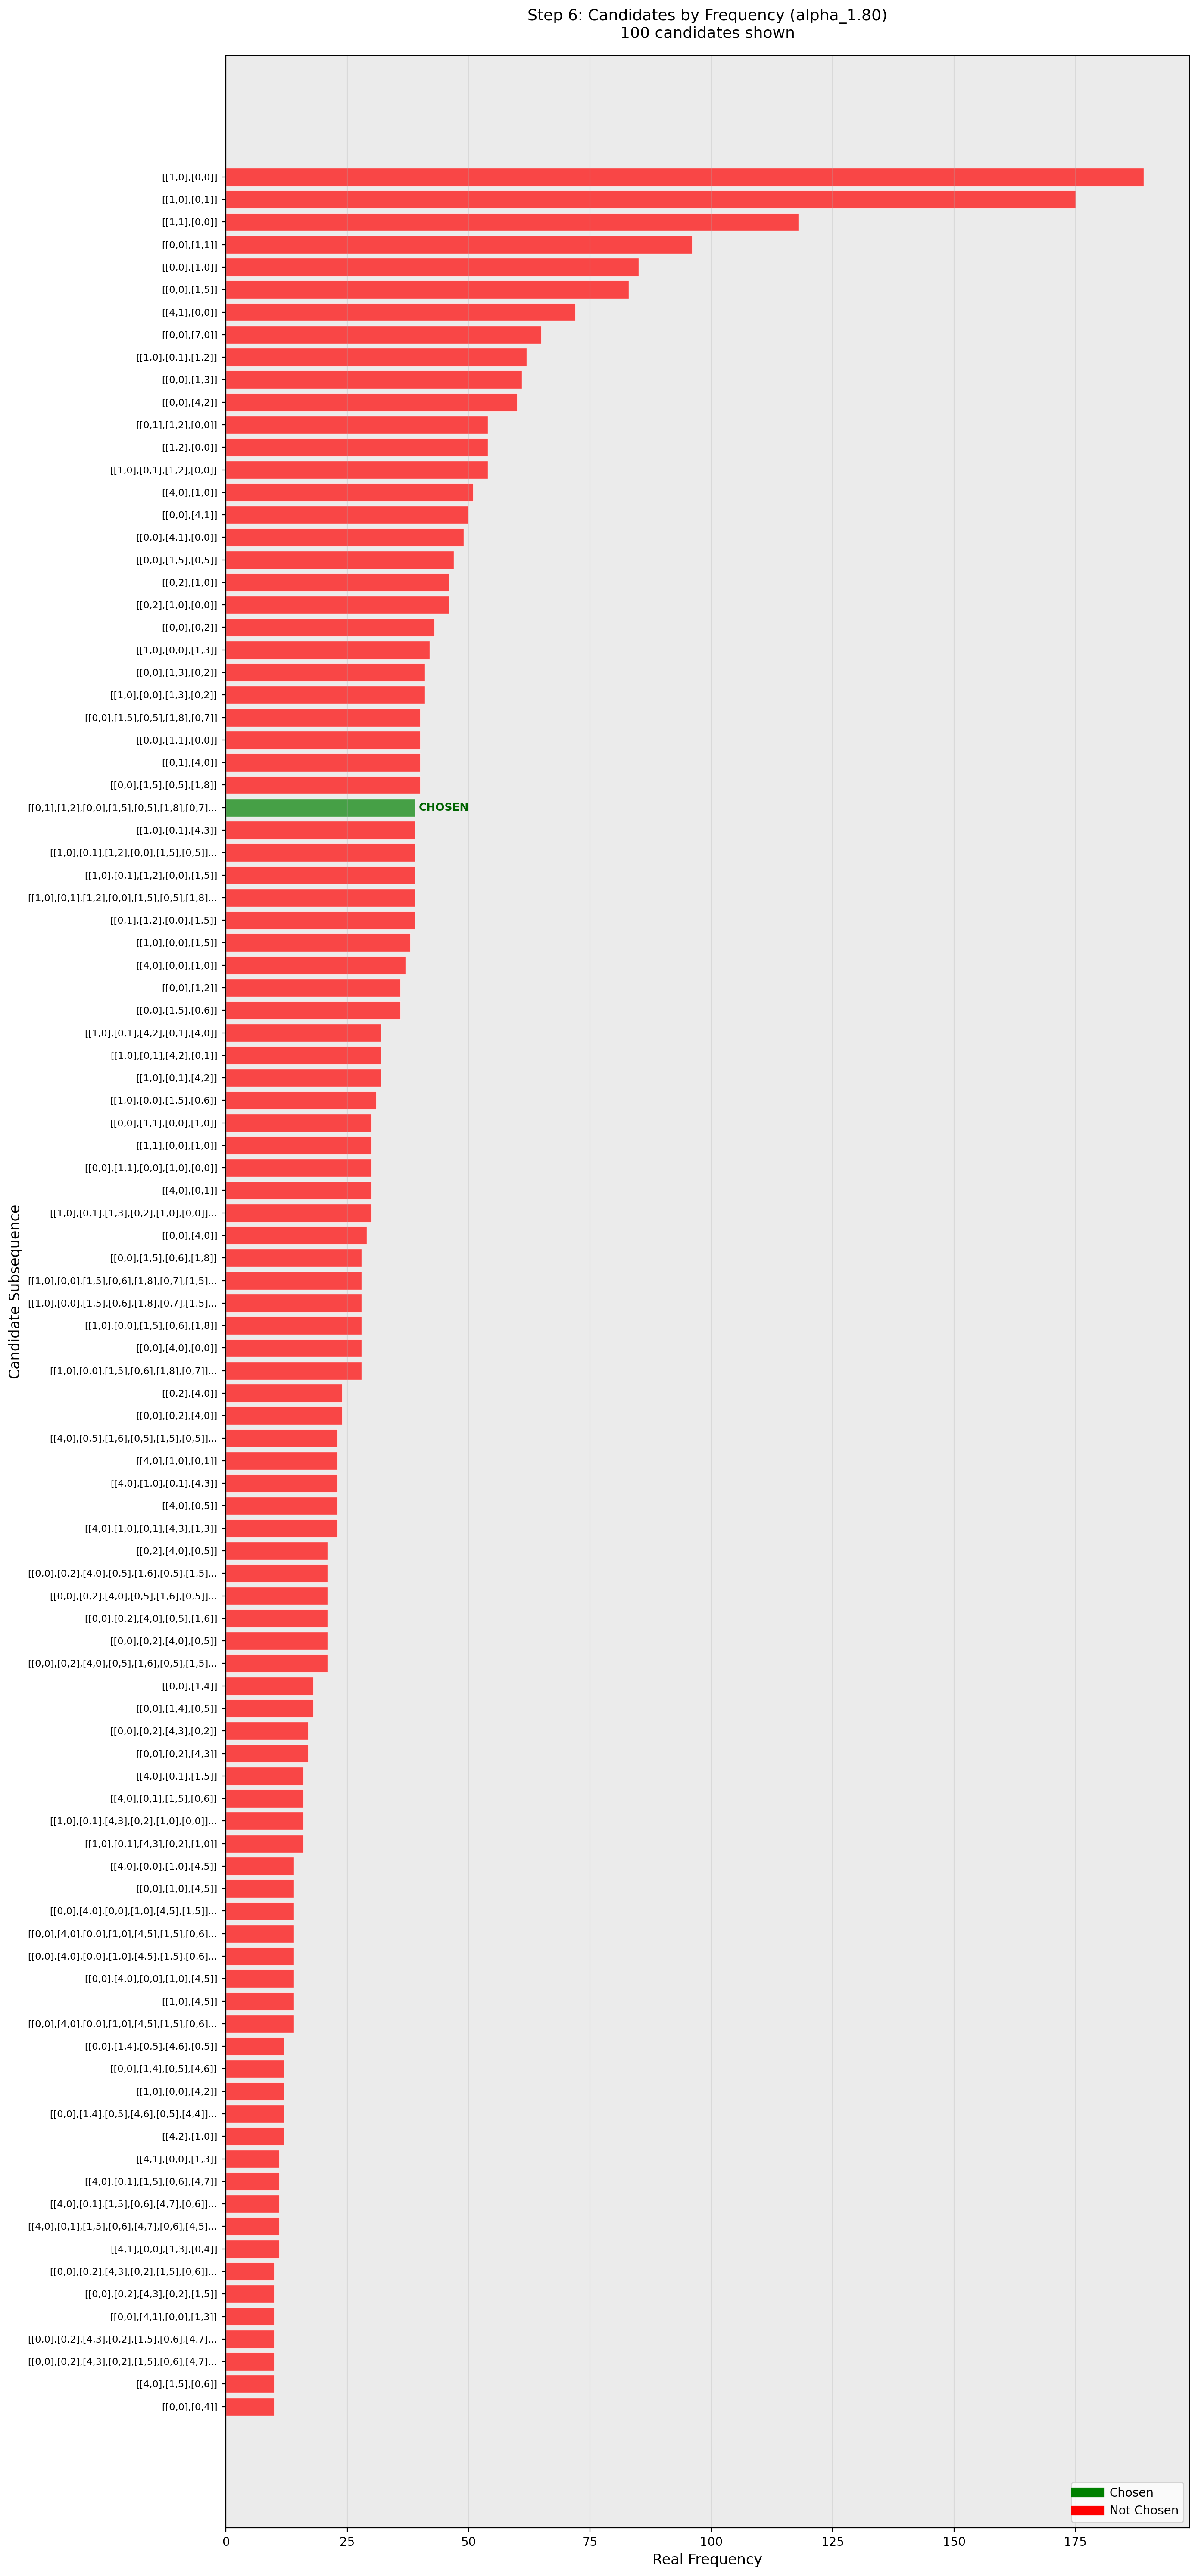
\includegraphics[width=0.72\textwidth]{images/frequency_snapshot_alpha_1.80_step_06.png}%
    }{%
        \fcolorbox{red}{white}{\parbox[c][0.14\textheight][c]{0.9\textwidth}{\centering\textcolor{red}{Placeholder figure\\\texttt{\detokenize{images/frequency_snapshot_alpha_1.80_step_06.png}}}}}%
    }
    \caption{Snapshot of candidate subsequences at proposal step 6 during training on the $\alpha = 1.80$ dataset (seed 42), ordered by raw frequency in descending order. The candidate adopted at this step under the MDL rule is highlighted in green; other candidates are shown in red.}
    \label{fig:rq1-frequency-snapshot-alpha-180-step-06}
\end{figure}

\begin{figure}[htbp]
    \centering
    \IfFileExists{images/mdl_snapshot_alpha_1.80_step_06.png}{%
        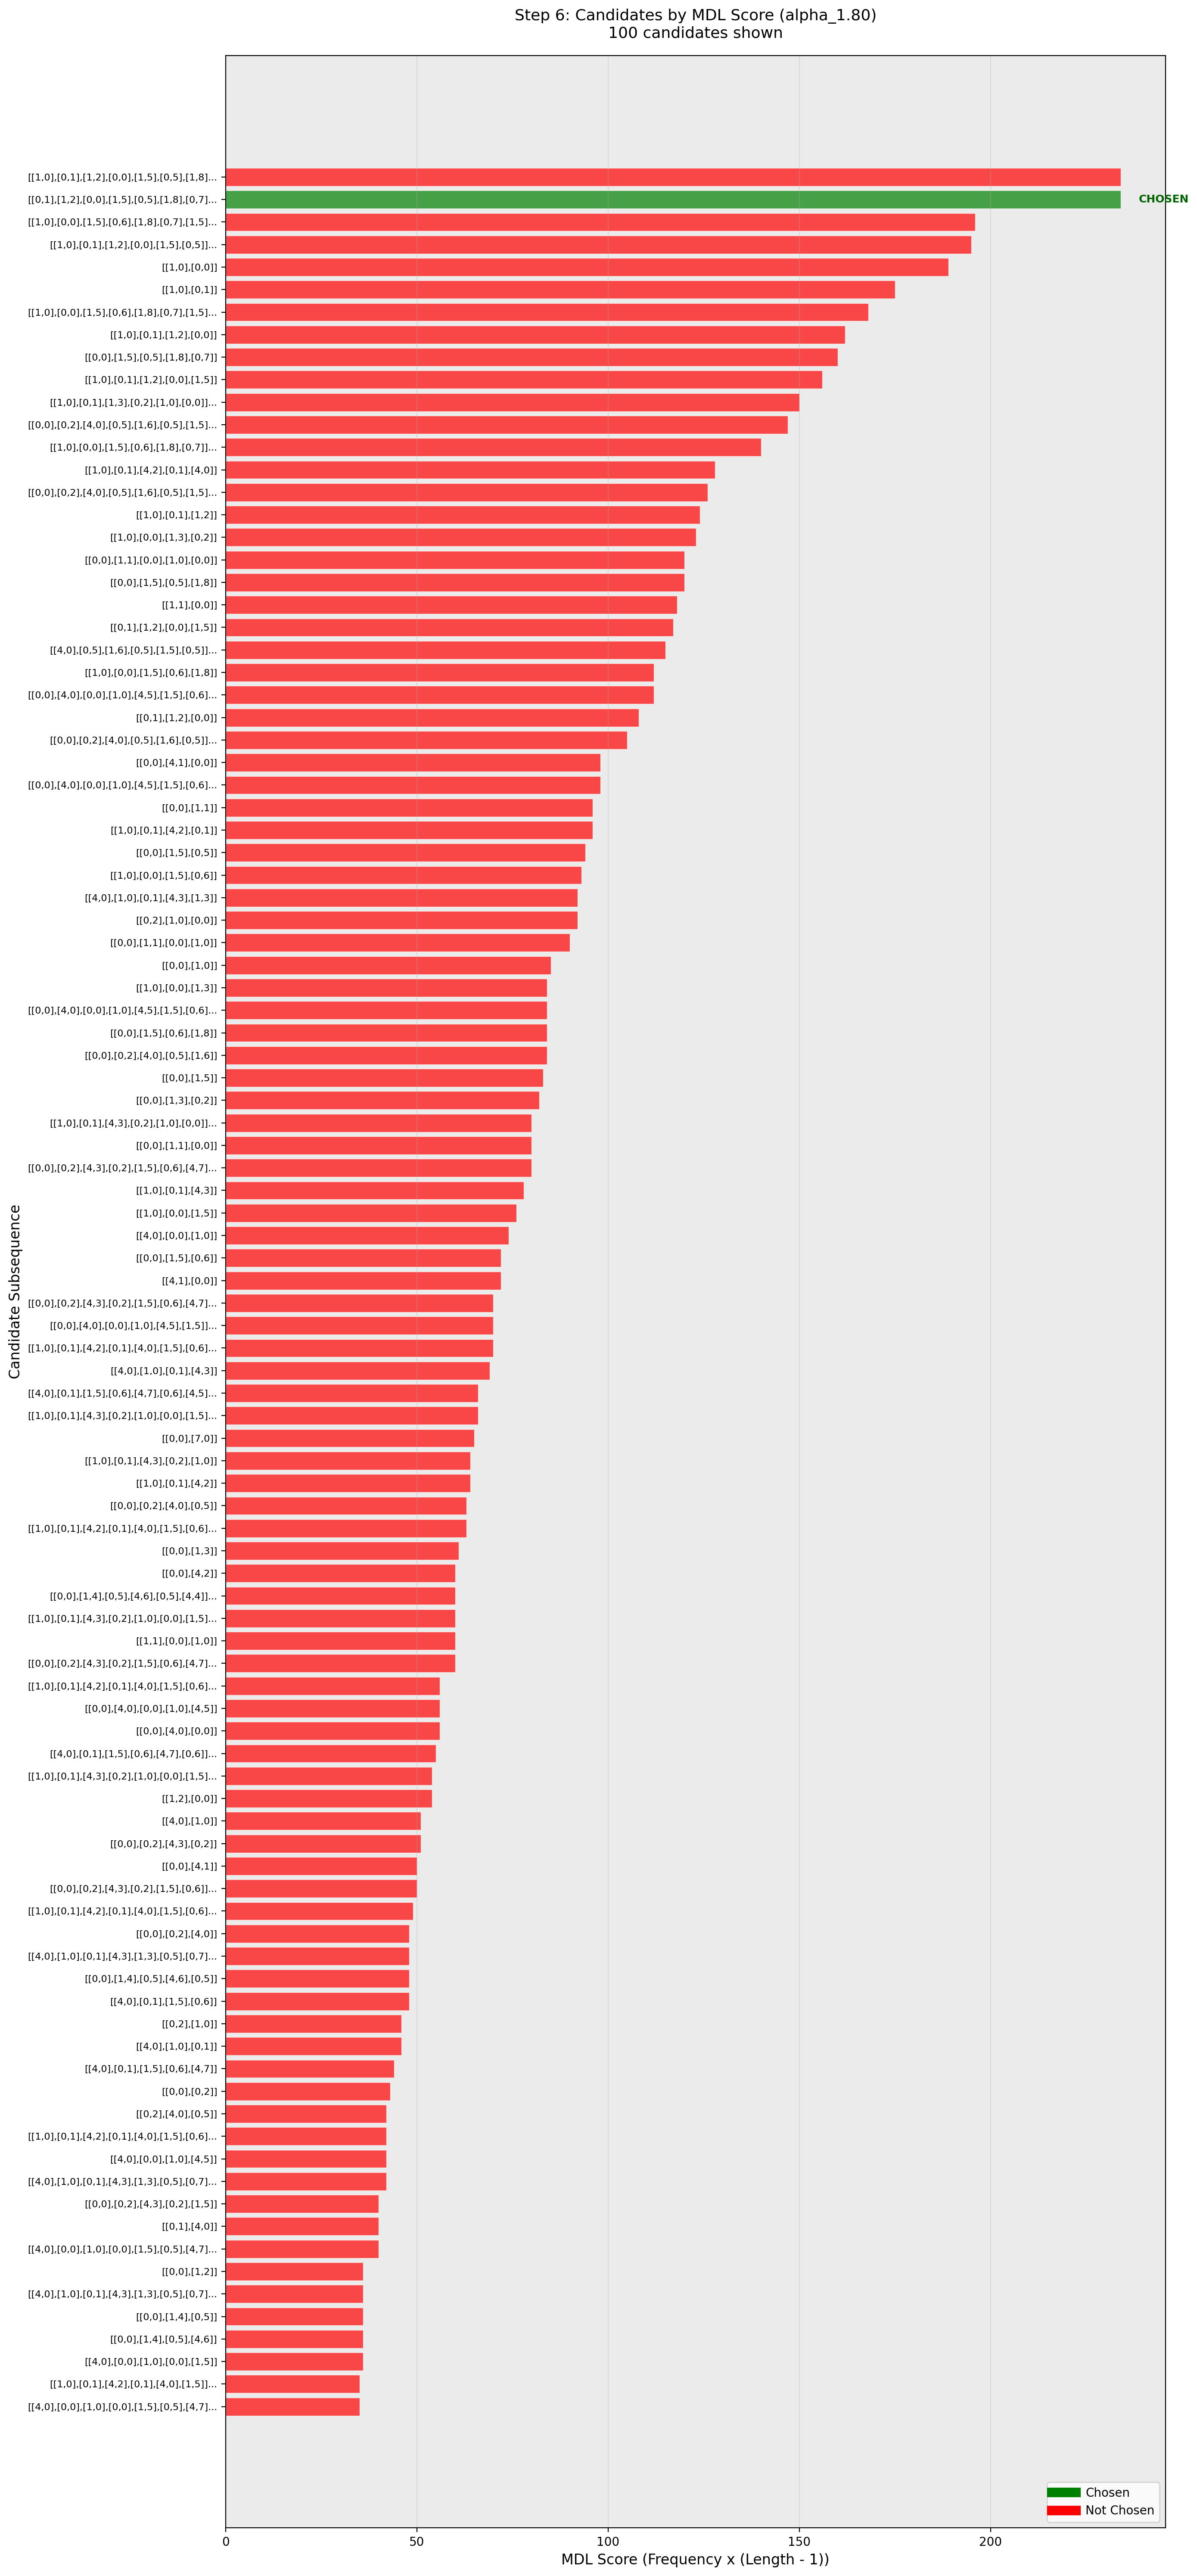
\includegraphics[width=0.72\textwidth]{images/mdl_snapshot_alpha_1.80_step_06.png}%
    }{%
        \fcolorbox{red}{white}{\parbox[c][0.14\textheight][c]{0.9\textwidth}{\centering\textcolor{red}{Placeholder figure\\\texttt{\detokenize{images/mdl_snapshot_alpha_1.80_step_06.png}}}}}%
    }
    \caption{Same candidate set as Figure~\ref{fig:rq1-frequency-snapshot-alpha-180-step-06}, but ordered by MDL score. The adopted candidate (green) sits at the top of the ranking, illustrating the deterministic MDL selection rule.}
    \label{fig:rq1-mdl-snapshot-alpha-180-step-06}
\end{figure}

The MDL score for a subsequence, as introduced in Chapter~\ref{ch:background}, is the product of frequency and length minus one. A subsequence with high raw frequency but very short length can therefore have a modest MDL score, because the ``length minus one'' factor is small. Conversely, a subsequence with moderate frequency but substantial length can have a large MDL score, because the length factor amplifies the frequency contribution. The divergence from the frequency ranking shows that PACE selects abstractions that will save tokens if adopted, rather than abstractions that merely correspond to the most common patterns.

There is one $\alpha$ regime where the picture is different. At $\alpha = 3.00$, the correlation between adoption decisions and raw frequency approaches statistical significance (Spearman $\rho = -0.626$, $p = 0.079$), and the correlation with length becomes significant ($\rho = -0.769$, $p = 0.026$). At this concentration, the pool of subsequences that see any meaningful frequency is so small that the MDL score essentially collapses onto the raw frequency ranking: the two signals largely agree, and the finer preference for compression-favouring candidates that MDL encodes at lower $\alpha$ becomes hard to distinguish from frequency.

\section{Discussion}
\label{sec:rq1-discussion}

The three analyses of this chapter converge on a coherent picture of how $\alpha$ shapes the internal structure of the emergent language.

The number of adopted abstractions follows a non-monotone pattern across $\alpha$, with a peak at $\alpha = 1.80$ in the intermediate regime and drops at both ends of the range. Section~\ref{sec:rq1-adoption-count} introduced this as a three-regime pattern; the rest of the chapter shows how the same regimes appear in compression and selection dynamics.

The compression dynamics of Section~\ref{sec:rq1-compression-dynamics} confirm that the intermediate $\alpha$ values produce the most compressed emergent languages, while high $\alpha$ ($\alpha = 3.00$) produces less compression in the same number of proposal steps. The three intermediate $\alpha$ values (0.00, 0.60, 1.80) reach comparable compression plateaus by the end of training; the difference is not in the final level of compression but in how many abstractions are used to achieve it. At low $\alpha$, compression is achieved with many small abstractions; at intermediate $\alpha$, with a smaller number of larger abstractions.

The MDL selection analysis of Section~\ref{sec:rq1-mdl-vs-frequency} tells us something important about the mechanism that produces these patterns. The deterministic MDL rule selects abstractions on the basis of a signal that combines frequency with length. This means that the emergent library is not merely a reflection of what the input distribution presents most often; it is a reflection of what compresses best. At high $\alpha$, however, this distinction breaks down: the top-ranked pairs are the only ones with enough frequency to matter, and MDL essentially reduces to a frequency-based ranking. This convergence of MDL and frequency at high $\alpha$ is the mechanism behind the small libraries observed in Section~\ref{sec:rq1-adoption-count}, and it foreshadows the difficulties that cross-population communication will show at high $\alpha$ in Chapter~\ref{ch:rq3}.

This tension mirrors a general account of why compositional structure emerges: frequent meanings are seen often enough to support holistic, memorised forms, whereas rare meanings in a large, sparse space can only be covered compositionally under limited exposure~\cite{gibson_how_2019,kirby_compression_2015}. Our three-regime result is the vocabulary-level counterpart: concentration must be high enough to drive reuse but low enough to preserve the diversity that makes abstraction worthwhile.

This aggregate pattern should be distinguished from frequency effects measured at the level of individual messages. Sevestre and Dupoux~\cite{sevestre_frequency_2025} report that frequent objects in a neural referential game become less compositionally encoded than rare objects, while earlier work shows that neural emergent languages can even violate Zipf's law of abbreviation by assigning longer messages to more frequent meanings~\cite{chaabouni_anti-efficient_2019}. Our claim is about a different axis: the size, compression, and selection dynamics of PACE's adopted symbolic vocabulary. On that axis, frequency and specialisation do not move together in the simple natural-language pattern.

The answer to RQ1 is therefore positive, but the effect of $\alpha$ is organised by regimes rather than by a single monotone slope. Library size, compression, and selection signal all point to the same interpretation: intermediate concentration provides enough repetition for useful patterns to score highly under MDL and enough residual diversity for further patterns to remain available. At the two extremes, one of those conditions breaks down, and the resulting language is less developed. PACE combines this symbolic pressure toward compression with an adaptive component: during joint training, the bandit selects for each scene whether to use a program containing abstractions or one built entirely from primitives.
